\documentclass[dia]{vcbook-float}
\usepackage{tikz-qtree}
\begin{document}
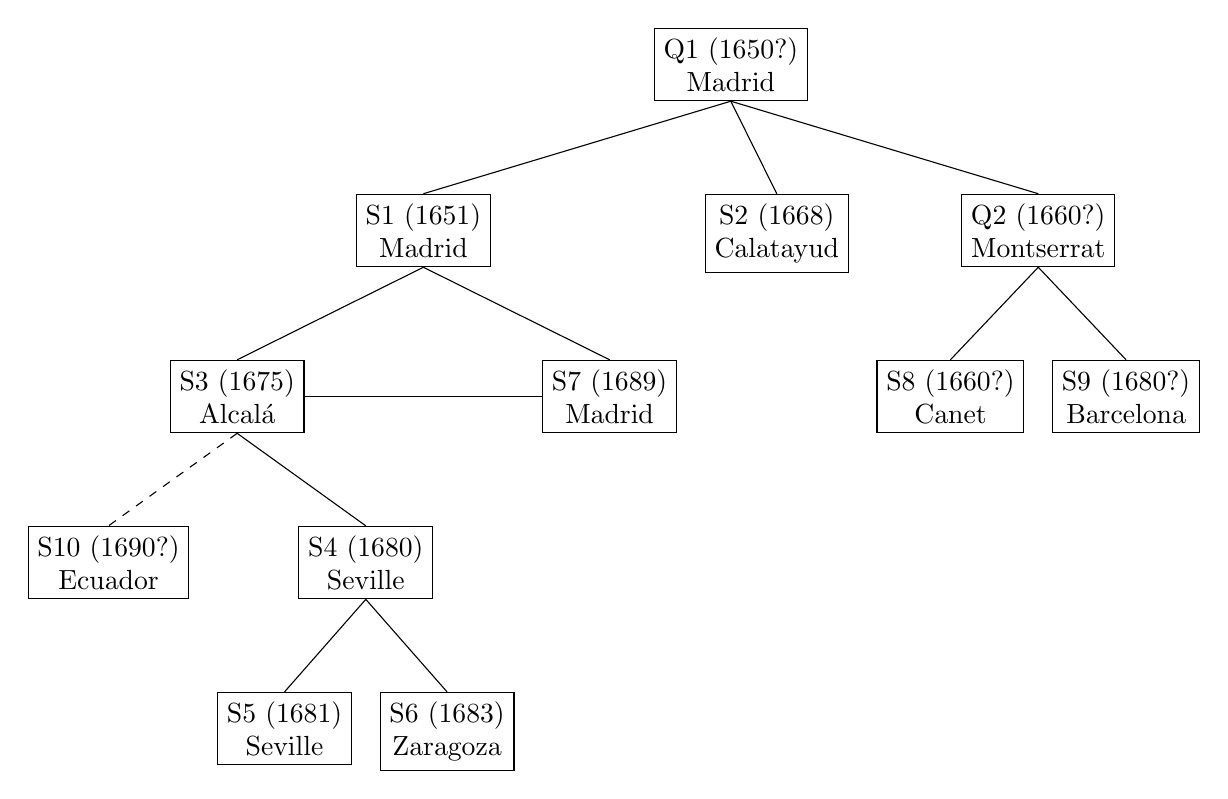
\begin{tikzpicture}
    \tikzset{every tree node/.style={draw,rectangle,align=center,anchor=north},
    level distance=6em, sibling distance=1em}
    \Tree [ .{Q1 (1650?)\\Madrid}
            [ .{S1 (1651)\\Madrid}
                [ .\node (S3) {S3 (1675)\\Alcalá};
                    \edge[dashed]; {S10 (1690?)\\Ecuador}
                    [ .{S4 (1680)\\Seville}
                        {S5 (1681)\\Seville} 
                        {S6 (1683)\\Zaragoza} ] ] 
               \node (S7) {S7 (1689)\\Madrid}; ]
           {S2 (1668)\\Calatayud} 
            [ .{Q2 (1660?)\\Montserrat}
                {S8 (1660?)\\Canet}
                {S9 (1680?)\\Barcelona} ] ] 
    \draw (S3) -- (S7);
\end{tikzpicture}
\end{document}

